\documentclass[../main.tex]{subfiles}
\begin{document}
\chapter{Sperimentazioni}

In questo capitolo vengono presentati gli esperimenti effettuati e le prestazioni ottenuti dallo script di conversione, successivamente i test fatti con Stratosphere IPS sulla creazione di modelli comportamentali per verificare l'accuratezza della conversione dei flows.

\section{Realizzazione di una piattaforma dedicata}

Per lo sviluppo del programma per la conversione dei file e per l'utilizzo di Stratosphere IPS è stata creata una piattaforma dedicata alla Security Analytics tramite l'utilizzo di \textit{VirtualBox} con una installazione del sistema operativo Ubuntu 16.04 LTS.


\begin{verse}
				\textbf{VirtualBox} è un software gratuito e open source per l'esecuzione di macchine virtuali che supporta Windows, GNU/Linux e macOS come sistemi operativi host ed è in grado di eseguire Windows, GNU/Linux, OS/2 Warp, BSD come ad esempio OpenBSD, FreeBSD e infine Solaris e OpenSolaris come sistemi operativi guest \cite{virtualbox}. 
\end{verse}


\section{Installazione Stratosphere IPS}
Sulla macchina virtuale è stato installato il framework di Stratospehere IPS. Di seguito i passaggi effettuati per l'installazione \cite{stf}.
\begin{itemize}
				\item Installazione del programma git 2.7.4 \cite{gitdef}
\begin{lstlisting}[language=bash]
 sudo apt install git
\end{lstlisting}
								Il pacchetto \textit{git} è necessario per interagire con il repository GitHub su cui è presente Stratosphere.
				\item Clonazione repository GitHub del framework
\begin{lstlisting}[language=bash]
 git clone https://github.com/stratosphereips/StratosphereTestingFramework
\end{lstlisting}
				\item Installazione del programma python-pip \cite{pipdef}
\begin{lstlisting}[language=bash]
 sudo apt install python-pip
\end{lstlisting}
Questo pacchetto serve per installare i pacchetti di Python e verrà usato per installare pacchetti successivi.
\end{itemize}
\begin{itemize}
				\item prettytable 0.7.2-3 \cite{prettytabledef}
\begin{lstlisting}[language=bash]
 sudo apt install python-prettytable
\end{lstlisting}
\textit{PrettyTable} è una libreria di Python usata per rappresentare tabelle ASCII.
				\item transaction 1.4.3-3 \cite{transactiondef}
\begin{lstlisting}[language=bash]
 sudo apt install python-transaction
\end{lstlisting}
								Questo pacchetto contiene l'implementazione delle transazioni per Python ed è usato principalmente da \textit{Zodb}.
				\item persistent 4.1.1-1build2 \cite{persistentdef}
\begin{lstlisting}[language=bash]
 sudo apt install python-persistent
\end{lstlisting}
								Il pacchetto contiene l'implementazione della persistenza dei dati per database come \textit{Zodb}.
				\item zodb 5.4.0 \cite{zodbdef}
\begin{lstlisting}[language=bash]
 sudo pip install zodb
\end{lstlisting}
È il database ad oggetti utilizzato dal framework.
				\item sparse 1.1-1.3build1 \cite{sparsedef}
\begin{lstlisting}[language=bash]
 sudo apt install python-sparse
\end{lstlisting}
Libreria che fornisce vettori multi dimensionali sparsi.
				\item dateutil 2.4.2-1 \cite{dateutildef}
\begin{lstlisting}[language=bash]
 sudo apt install python-dateutil
\end{lstlisting}
								Modulo che fornisce un'estensione al modulo standard di Python \textit{datetime}.

\end{itemize}

\section{Installazione di Argus}

Per generare i netflow dal traffico di rete è necessario avere una istanza di Argus sul computer. I seguenti passaggi sono necessari per la corretta installazione di Argus \cite{stf}.
\begin{itemize}
				\item libpcap 1.7.4-2
\begin{lstlisting}[language=bash]
 sudo apt install libpcab-dev
\end{lstlisting}
\item bison 3.0.4
\begin{lstlisting}[language=bash]
 sudo apt install bison
\end{lstlisting}
\item flex 2.6.0-11
\begin{lstlisting}[language=bash]
 sudo apt install flex
\end{lstlisting}
\item Installazione dell'ultima versione di argus 3.0.8.2 dal sito\\ http://qosient.com/argus/dev/argus-latest.tar.gz
\item Installazione dell'ultima versione di argus-client 3.0.8.2 dal sito\\ http://qosient.com/argus/dev/argus-clients-latest.tar.gz
\end{itemize}

\section{Utilizzo del programma STF\\}
In questa sezione viene presentato il framework di Stratoshpere le la creazione dei modelli comportamentali, STF. 

Per eseguire il programma si usa il comando
\begin{lstlisting}[language=bash]
	./stf.py
\end{lstlisting}
La figura ~\ref{fig:homestf} mostra l'interfaccia a console del programma STF
\begin{figure}[H]
				\centering
				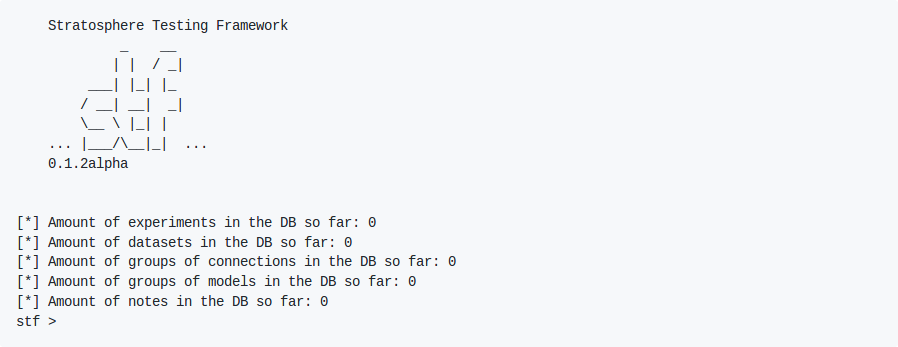
\includegraphics[scale=0.4]{homestf.png}
				\caption{Interfaccia a console di STF}
				\label{fig:homestf}
\end{figure}

Per caricare un dataset si utilizza il comando
\begin{lstlisting}[language=bash]
	datasets -c /absolute/path/file.binetflow	
\end{lstlisting}

Per generare la connessione si utilizza il comando
\begin{lstlisting}[language=bash]
	connections -g	
\end{lstlisting}

Infine, per generare i modelli, il comando
\begin{lstlisting}[language=bash]
	models -g	
\end{lstlisting}

Per visualizzare il behavioral model si utilizza il comando
\begin{lstlisting}[language=bash]
	models -L [id]	
\end{lstlisting}

\end{document}

\section{Prestazioni}

Come visto nel capitolo 4, il programma di conversione proposto è efficiente. In questa sezione vengono effettuati dei \textit{benchmark} per analizzarne le prestazioni e studiare la scalabilità di una soluzione che prevede l'utilizzo di più CPU in parallelo.

\subsection{Benchmark}

Per misurare la velocità del programma sono stati usati 3 dataset:
\begin{itemize}
				\item 10 giorni di flows di dimensione totale 1,7 GB
				\item 5 giorni di flows di dimensione totale 700 MB
				\item 1 giorno di flows di dimensione totale 70 MB
\end{itemize}

Le misure sono state realizzate con il programma /usr/bin/time. I grafici sono stati creati con il programma GNU Octave per GNU/Linux \cite{octave}.

Il computer su cui sono stati effettuati i benchmark ha le seguenti caratteristiche:
\begin{itemize}
				\item Linux Mint 19 Cinnamon
				\item Kernel 4.15.0-20-generic
				\item Processore Intel Core i7-3770 @ 3.40GHz 
				\item RAM 8 GB
				\item HDD 2 TB 7200 RPM
\end{itemize}

I benchmark sono stati effettuati convertendo il dataset con l'algoritmo visto nel capitolo 4. I benchmark sono stati ripetuti in funzione del numero di core disponibili sulla CPU. I tempi di esecuzione sul dataset di 1,7 GB sono:
\begin{itemize}
				\item 1 core: 11.35.46
				\item 2 core: 6.02.65
				\item 3 core: 4.12.62
				\item 4 core: 3.09.79
				\item 5 core: 3.04.47
				\item 6 core: 3.04.66
				\item 7 core: 2.59.22
				\item 8 core: 2.59.33
\end{itemize}

Come è possibile constatare dai risultati, per i primi 4 core si ha un guadagno lineare, mentre gli ultimi 4 forniscono un miglioramento non più lineare. Questo è dovuto al numero di core della CPU usata per i benchmark, l'i7-3770 ha 4 core fisici e 4 virtuali sfruttando la tecnologia \textit{Hyper Threading} \cite{hyperthreading} di Intel.

La figura ~\ref{fig:tempoCore} rappresenta il grafico che è stato costruito sui risultati dell'esecuzione dei 3 diversi dataset: ha sull'asse delle $x$ il numero di core e sull'asse delle $y$ il tempo impiegato per convertire i file. Il colore blu identifica il dataset di dimensione 1,7 GB, il colore rosso 700 MB e quello verde 70 MB. Come si può vedere il tempo impiegato scende in modo quasi lineare per i primi quattro core nel dataset più grosso. Il grafico verde rimane quasi costante perchè per dataset di dimensioni molto ridotte aggiungere core è quasi ininfluente.

\begin{figure}[H]
				\centering
				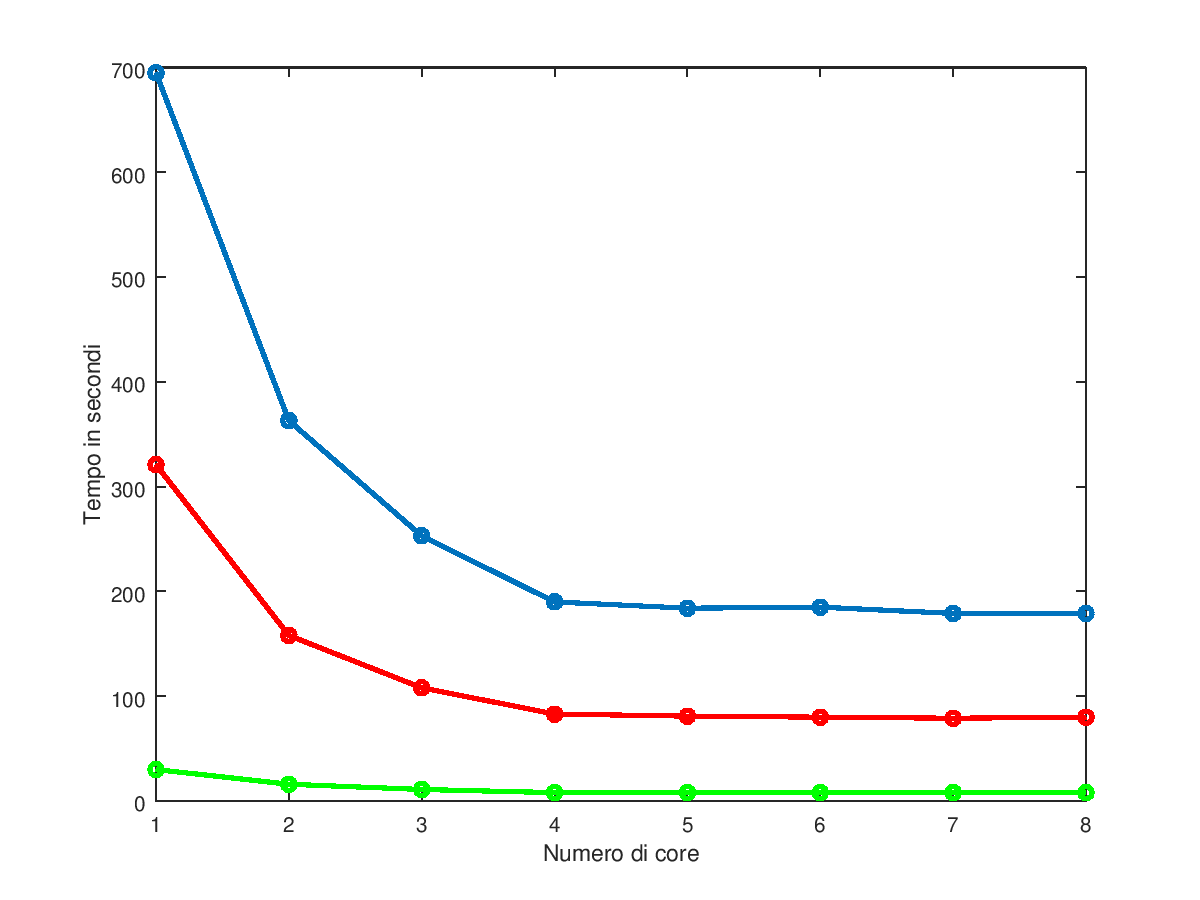
\includegraphics[scale=0.7]{graph1.png}
				\caption{Andamento del tempo in funzione del numero di core}
				\label{fig:tempoCore}
\end{figure}

\subsection{Metrica delle prestazioni parallele}

Sia $T$(p) il tempo di esecuzione in secondi di un certo algoritmo su $p$ processori. Di conseguenza sia $T$(1) il tempo di esecuzione del codice parallelo su 1 processore.
La \textit{misura di scalabilità} o \textit{speedup} relativo di un algoritmo parallelo eseguito su \textit{p} processori si calcola come:
\begin{center}
\begin{math}
S(p) = \frac{T(1)}{T(p)}
\end{math}
\end{center}
In un sistema ideale, in cui il carico di lavoro potrebbe essere perfettamente partizionato su $p$ processori, lo speedup relativo dovrebbe essere uguale a $p$. In questo caso si parla di speedup lineare.

Con i risultati ottenuti in precedenza si è calcolato lo speedup per ogni numero di core. La figura seguente mostra l'andamento dello speedup relativo in funzione del numero di core. Si vede come la curva è inizialmente prossima ad uno speedup lineare, poi si ha un punto di saturazione dovuto ai costi di comunicazioni tra i vari cori che cominciano a prevalere sugli altri costi. Si ha che
\begin{center}
\begin{math}
				\lim_{p\rightarrow \infty } S(p)=0
\end{math}
\end{center}
C'è una soglia, che dipende dall'algoritmo e dall'architettura del sistema, oltre la quale è controproducente aumentare il numero di core. La figura ~\ref{fig:speedup} descrive l'andamento dello speedup con i risultati ottenuti.

\begin{figure}[H]
				\centering
				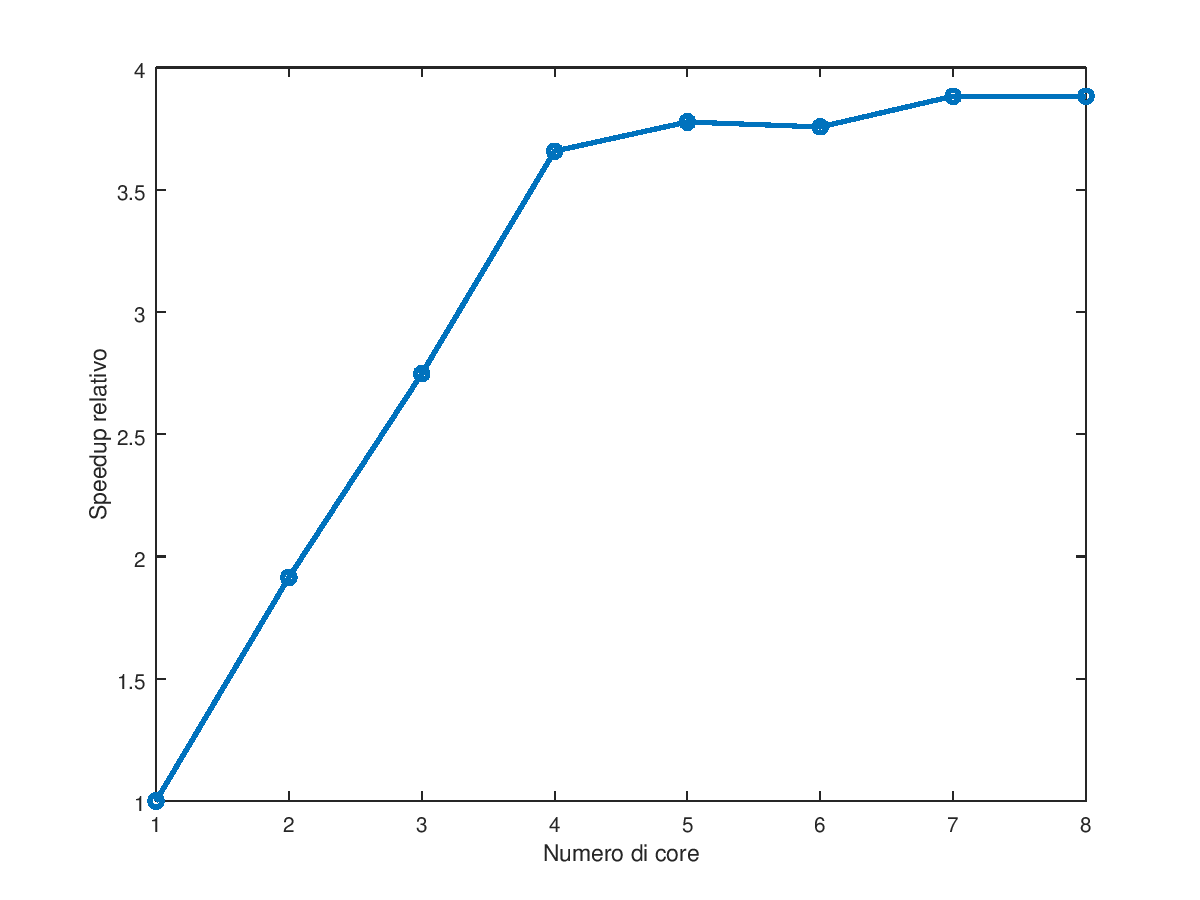
\includegraphics[scale=0.7]{graph2.png}
				\caption{Andamento dello speedup in funzione del numero di core}
				\label{fig:speedup}
\end{figure}

Si definisce \textit{efficienza} il rapporto
\begin{center}
\begin{math}
E(p) = \frac{S(p)}{p}
\end{math}
\end{center}

Idealmente, se l'algoritmo avesse uno speedup lineare, si avrebbe 
\begin{math}
E(p) = 1.
\end{math}
Nella pratica $E(1) = 1$ mentre $E(p)$, per $p > 1$, è una funzione decrescente. 
Più l'efficienza si allontana da 1, peggio stiamo sfruttando le risorse di calcolo disponibili nel sistema parallelo.

La figura ~\ref{fig:efficienza} mostra l'andamento dell'efficienza del programma di conversione al variare del numero di processori. Usando quattro core si ha un'efficienza leggermente maggiore di 0.9 mentre con l'aggiunta di altri core si può notare chiaramente come l'efficienza cali.
\begin{figure}[H]
				\centering
				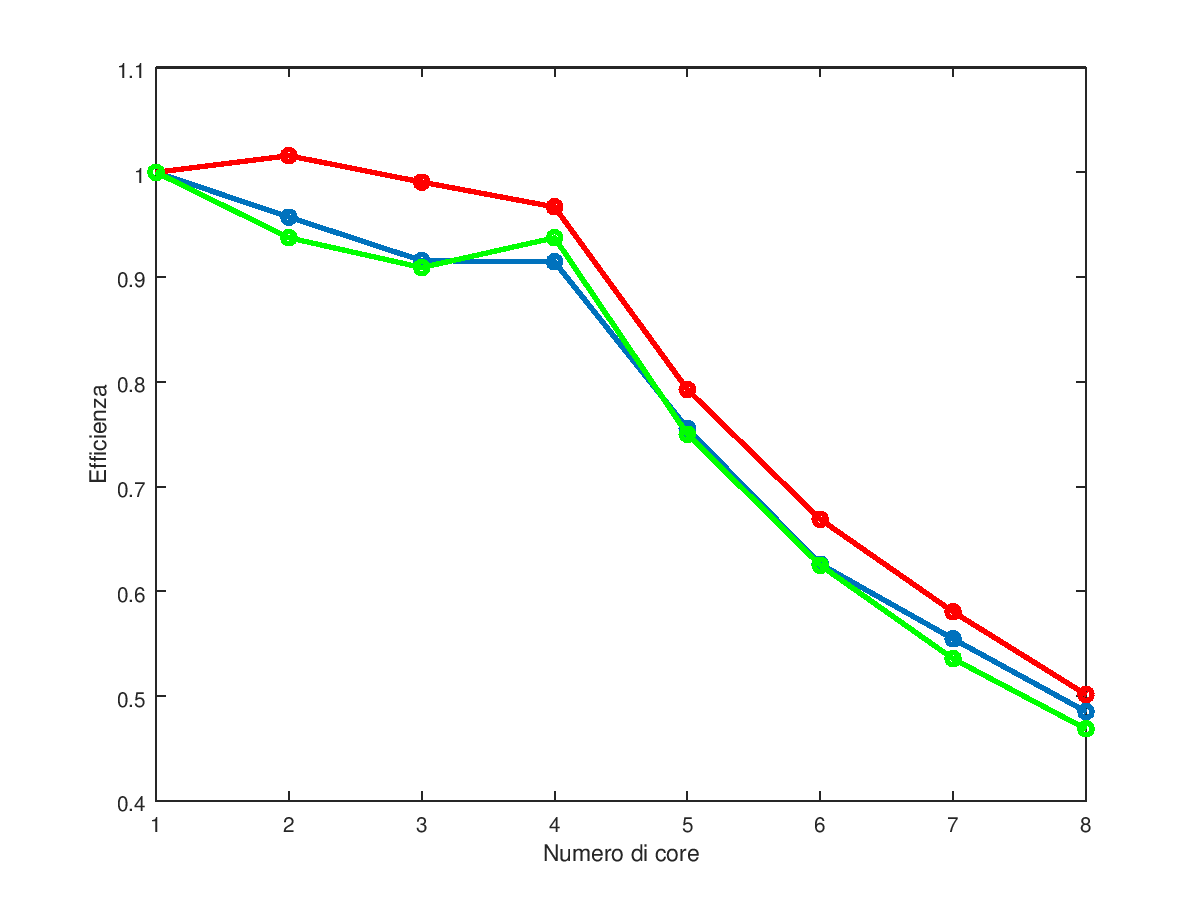
\includegraphics[scale=0.7]{graph3.png}
				\caption{Andamento dell'efficienza in funzione del numero di core}
				\label{fig:efficienza}
\end{figure}
Per determinare il numero ottimale di core da utilizzare per un certo algoritmo bisogna cercare il numero di core con efficienza e speedup maggiore. Si osserva che:
\begin{itemize}
				\item $E(p)$ ha il massimo per $p = 1$
				\item $S(p)$ ha il massimo in corrispondenza del punto di saturazione, in cui però l'efficienza è piuttosto bassa
\end{itemize}
Per trovare il numero ottimo si usa la \textit{funzione di Kuck}
\begin{center}
\begin{math}
				F(p) = E(p)S(p)
\end{math}
\end{center}
Questa funzione restituisce un numero che mette in relazione l'efficienza e lo speedup. Il numero ottimale di core $p_{F}$ con cui eseguire un algoritmo è il numero in corrispondenza del massimo della funzione di Kuck.
\begin{center}
\begin{math}
				p_{F} = argmaxF(p)
\end{math}
\end{center}
Nella figura ~\ref{fig:kuck} è rappresentata la funzione di Kuck 
\begin{figure}[H]
				\centering
				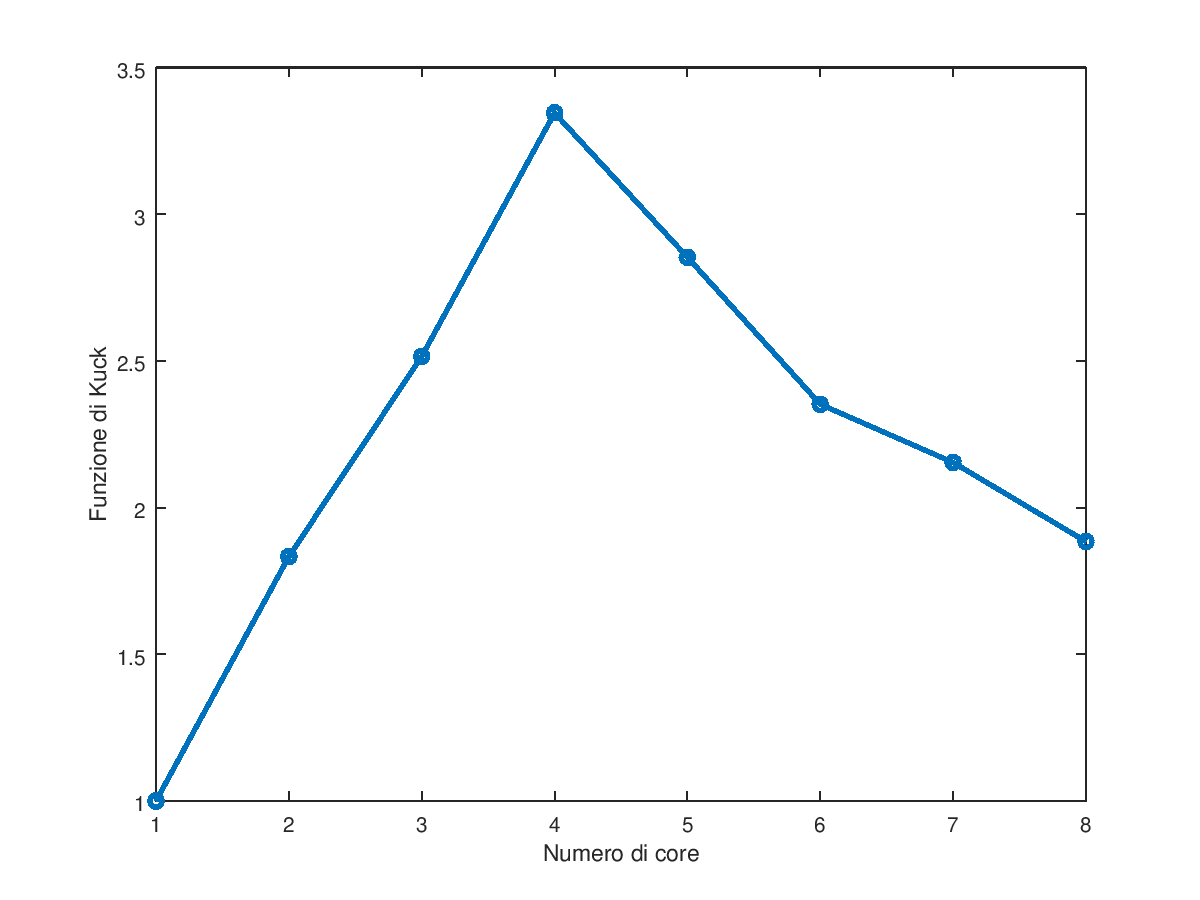
\includegraphics[scale=0.7]{graph4.png}
				\caption{Funzione di Kuck al variare del numero di core}
				\label{fig:kuck}
\end{figure}
La conversione in parallelo risulta molto efficiente, intorno allo 0.9. Con gli esperimenti effettuati ci si aspetta uno speedup lineare sul numero di core fisici.
Utilizzando un solo core la conversione impiega 12 minuti, mentre con quattro core si divide in quattro il tempo arrivando a 3 minuti. Le CPU di nuova generazione come AMD Ryzen vantano 32 core fisici e 32 virtuali, con questo numero di core fisici ci si può aspettare di dividere il tempo per 32, arrivando ad effettuare la conversione in 23 secondi.

\section{Conversione}
Per controllare se la conversione viene effettuata correttamente si è usato il software Stratosphere IPS per creare e utilizzare dei modelli impiegati per fare \textit{anomaly detection} su del traffico di rete. I flows sono stati convertiti nel formato compatibile da Argus ad nProbe e infine di nuovo ad Argus per controllare che non ci siano delle perdite di informazioni vitali che alterino il funzionamento dell'IDPS.

La figura ~\ref{fig:processoConversione} descrive il processo di conversione. Ad ogni conversione effettuata è prevista una perdita di informazioni dovuta al tipo di campi utilizzati nei diversi formati e alla loro formattazione.

\begin{figure}[H]
				\centering
				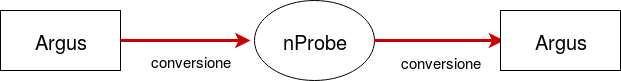
\includegraphics[scale=0.5]{conversion.png}
				\caption{Processo di conversione}
				\label{fig:processoConversione}
\end{figure}
In questa sezione si è utilizzato slips per verificare che la conversione dei file di flows sia corretta. È stato usato un flow dato in input a slips per rilevare del traffico malevolo, successivamente convertito in un altro formato e riconvertito per verificare che l'output sia identico pre e post conversione.
I flows e i modelli comportamentali utilizzati per il test sono stati presi dal repository GitHub di slips \cite{slips}.

Nel test effettuato si è utilizzato il file "2016-11-4\_win11.binetflow" con il seguente comando
\begin{lstlisting}
cat test-flows/Malicious/2016-11-4_win11.binetflow | ./slips.py -f models/ -d
\end{lstlisting}
l'output di slips è rappresentato in figura ~\ref{fig:outputSlips}. Sono stati rilevati 3 indirizzi IP malevoli dal file di flow dato in input.
\begin{figure}[H]
				\centering
				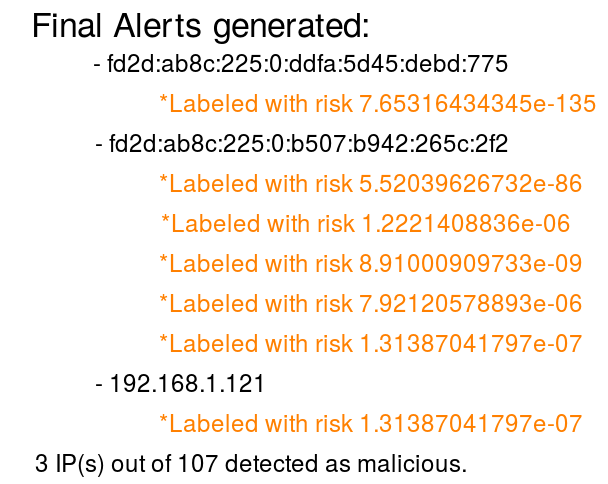
\includegraphics[scale=0.5]{slips.png}
				\caption{Output slips}
				\label{fig:outputSlips}
\end{figure}


\end{document}
